%%% Article Template
%%% Set Document layout
\documentclass[final, 12pt]{article}

%%%%%%%%%% Set Name, Subject, Date ...
\newcommand{\toppic}{Analysis}
\newcommand{\mytitle}{Analysis}
\newcommand{\workingDate}{12.01.2023}
\newcommand{\userName}{Jonathan Mayer}
%%
\usepackage{options}

%%%%%%%%%% Begin the document
\begin{document}  
\begin{center}
    {\textbf {\huge \mytitle}}\\[5mm]   % titel
    {\large \userName} \\[5mm]          % User Name
    \workingDate\\                      % Working Date
\end{center} %%%%%%%%%% Titel %%%%%%%%%%%%%%

%%
\section{Begriffe}
\begin{center}
    \begin{tblr}{ll}
        \textbf{Symbol}         & \textbf{Bedeutung} \\ \hline[1.5pt]
         $R$                    & Relation \\\hline
         $\in/ \notin$          & Element / kein Element von \\\hline
         $\forall / \nexists$   & für alle / für kein \\\hline
         $\exists$              & Existenzquantor, mindestens ein \\\hline
         $\exists !$            & Anzahlquantor, genau ein \\\hline
         $A \subset B$          & echte Teilmenge, $a \in A \land a,b \in B:\exists b\notin A$\\ \hline
         $A \subseteq B$        & Teilmenge $a \in A \land a,b \in B$ \\\hline
         $]1,3[$, $(1,3)$       & $1<x<3$ \\\hline
         $[1,3]$                & $1\leq x \leq 3$ \\\hline
         $\Rightarrow$          & genau dann wenn \\\hline
         $\Leftrightarrow$      & aus Aussage A folg B und umgekehrt \\\hline
         $\rightarrow$          & Abbildungsvorschrift für Mengen \\\hline
         $\mapsto$              & Abbildungsvorschrift für Elemente \\\hline
         $\circ$                & Komposition / Verkettung von Funktionen \\\hline
         $\land\ /\ \lor$       & und / oder \\\hline
         Lemma                  & Hilfssatz \\\hline
         $\overline{z}, \ z^*$  & konjungiert komplexe Zahl \\\hline
         $\preccurlyeq$         & beliebiges Symbol \\\hline
         $\stackrel{?}{=}$      & zu zeigen \\\hline
         $\stackrel{!}{=}$      & soll erfüllt sein um ... zu zeigen \\\hline
         $:=, \equiv$           & definiere \\\hline
         $\cup,\cap, /$         & Vereinigung, Durchschnitt, Subtrahiert \\\hline
         disjunkt               & $A \cap B = \{\}$ \\\hline
         infimum \\\hline
         supremum \\\hline

    \end{tblr}
\end{center}




%%
\section{Stetigkeit}

\textbf{Definition Stetigkeit:}\\
$\forall \epsilon > 0 :\exists \delta > 0 : |x-a|<\delta : |f(x)-f(a)|<\epsilon$\\
$\forall \epsilon > 0 :\exists \delta > 0 : f(U_{\delta}(a) \subseteq U_{\epsilon}(f(a)))$\\
$\forall \epsilon > 0\  \exists \delta >0 : \text{sodass aus } |x-a|<\delta \text{ stets } |f(x)-f(a)|<\epsilon \text{ folgt}$\\

\textbf{Definition Unstetigkeit:} $\exists \epsilon > 0 \forall\  \delta > 0 :\exists x \in D : |x-x_0|< \delta \wedge |f(x)-f(x_0)|>\epsilon$

\subsection{links-rechtsseitiger Grenzwetz:}

$\lim\limits_{x\to x_0^-}f(x) = \lim\limits_{x\to x_0^+} f(x)$

$x_0$ wird von rechts und links angenähert. Sind beide Grenzwerte gleich ist die Funktion stetig.


\subsection{$\epsilon - \delta$ Kriterium}

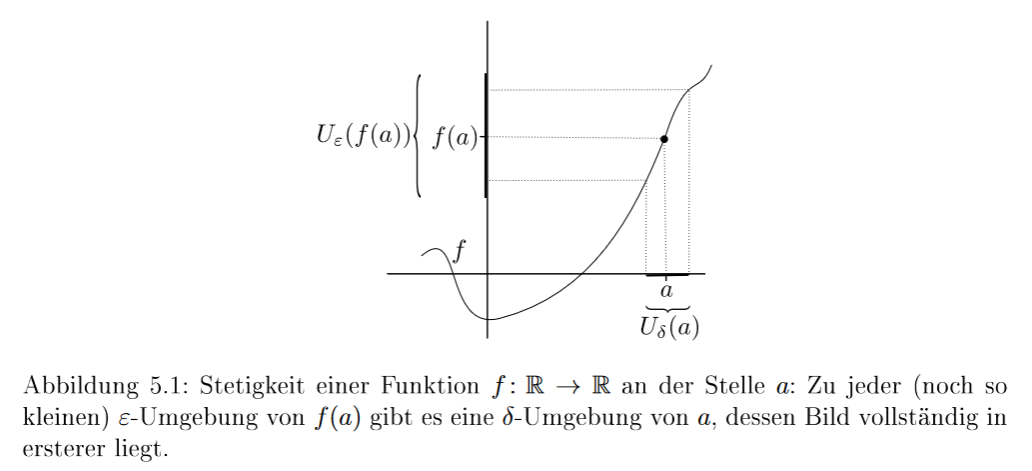
\includegraphics[width= \textwidth]{./pictures/Stetigkeit.png}
$\epsilon$ quer darf nach oben abgeschätz werden.
Zuerst delta ausrechnen
dann Beweis nochmal schön hinschrieben.\\

$|x-a|<\delta$\\
$|f(x)-f(a)|< \epsilon|$\\

$\epsilon$ darf gewählt werden

Nicht Stetigkeit beweisen:\\
>links und rechtsseitiger Grenzwert\\
>epsilon delta Kriterium

-->

$\exists \epsilon > 0 :\forall \delta >0 \exists x |x-x_0| < \delta \vee |f(x)-f(x_0) > \epsilon|$



%%% Verzeichnisse
\newpage
%\listoftables
%\listoffigures
%\printbibliography{}
%%%%%% Document end
\end{document}     %%% End the document


